% Pengaturan ukuran teks dan bentuk halaman dua sisi
\documentclass[12pt]{book}

% Pengaturan ukuran halaman dan margin
\usepackage[a4paper,top=30mm,left=30mm,right=20mm,bottom=25mm]{geometry}

% Pengaturan ukuran spasi
\usepackage[singlespacing]{setspace}

% Pengaturan caption untuk tabel
\usepackage{caption}

% Judul dokumen
\title{Proposal Tugas Akhir ITS}
\author{Musk, Elon Reeve}

% Pengaturan detail pada file PDF
\usepackage[pdfauthor={\@author},bookmarksnumbered,pdfborder={0 0 0}]{hyperref}


% Pengaturan ukuran indentasi
\setlength{\parindent}{2em}

% Package lainnya
\usepackage{changepage}
\usepackage{etoolbox} % Mengubah fungsi default

% Pengaturan jenis karakter
\usepackage[utf8]{inputenc}

\usepackage[style=ieee, backend=biber]{biblatex}
\usepackage{enumitem} % Pembuatan list
\usepackage{lipsum} % Pembuatan template kalimat
\usepackage{graphicx} % Input gambar
\usepackage{longtable} % Pembuatan tabel
\usepackage[table,xcdraw]{xcolor} % Pewarnaan tabel
\usepackage{eso-pic} % Untuk menggunakan background image di halaman
\usepackage{txfonts} % Font times
\usepackage{changepage} % Pembuatan teks kolom
\usepackage{multicol} % Pembuatan kolom ganda
\usepackage{multirow} % Pembuatan baris ganda
\usepackage{tabularx} % Untuk mengatur kolom, seperti grid pada CSS
\usepackage{wrapfig}
\usepackage{float}

% Pengaturan format daftar isi, daftar gambar, dan daftar tabel
\usepackage[titles]{tocloft}
\setlength{\cftsecindent}{2em}
\setlength{\cftsubsecindent}{2em}
\setlength{\cftbeforechapskip}{1.5ex}
\setlength{\cftbeforesecskip}{1.5ex}
\setlength{\cftbeforetoctitleskip}{0cm}
\setlength{\cftbeforeloftitleskip}{0cm}
\setlength{\cftbeforelottitleskip}{0cm}
\renewcommand{\cfttoctitlefont}{\hfill\Large\bfseries} % command untuk membuat heading bold dan besar
\renewcommand{\cftaftertoctitle}{\hfill}
\renewcommand{\cftloftitlefont}{\hfill\Large\bfseries}
\renewcommand{\cftafterloftitle}{\hfill}
\renewcommand{\cftlottitlefont}{\hfill\Large\bfseries}
\renewcommand{\cftafterlottitle}{\hfill}

% Definisi untuk "Hati ini sengaja dikosongkan"
\patchcmd{\cleardoublepage}{\hbox{}}{
  \thispagestyle{empty}
  \vspace*{\fill}
  \begin{center}\textit{[Halaman ini sengaja dikosongkan]}\end{center}
  \vfill}{}{}

  % Pengaturan penomoran halaman
\usepackage{fancyhdr}
\fancyhf{}
\renewcommand{\headrulewidth}{0pt}
\pagestyle{fancy}
\fancyfoot[C,CO]{\thepage}
\patchcmd{\chapter}{plain}{fancy}{}{}
\patchcmd{\chapter}{empty}{plain}{}{}

% Pengaturan format judul bab
\usepackage{titlesec}
\renewcommand{\thesection}{\thechapter.\arabic{section}}
\titleformat{\chapter}[hang]{\centering\bfseries\large}{BAB\ \arabic{chapter}\ }{0ex}{\vspace{0ex}\centering}
\titleformat*{\section}{\large\bfseries}
\titleformat*{\subsection}{\normalsize\bfseries}
\titlespacing{\chapter}{0ex}{0ex}{4ex}
\titlespacing{\section}{0ex}{1ex}{0ex}
\titlespacing{\subsection}{0ex}{0.5ex}{0ex}
\titlespacing{\subsubsection}{0ex}{0.5ex}{0ex}
\setcounter{secnumdepth}{3} % Untuk memberi penomoran pada \subsubsection

\counterwithin{figure}{chapter}
\counterwithin{table}{chapter}

% Mengganti figure dan table menjadi gambar dan tabel
\renewcommand{\figurename}{Gambar}
\renewcommand{\tablename}{Tabel}

% Tambahkan format tanda hubung yang benar di sini
\hyphenation{
  ro-ket
  me-ngem-bang-kan
  per-hi-tu-ngan
}

% Menambahkan resource daftar pustaka
\addbibresource{pustaka/pustaka.bib}

% Isi keseluruhan dokumen
\begin{document}
  % Nomor halaman pembuka dimulai dari sini
  \pagenumbering{roman}

  % Atur ulang penomoran halaman
  \setcounter{page}{1}

  % Sampul Bahasa Indonesia
  \newcommand\covercontents{sampul/konten-id.tex}
  \AddToShipoutPictureBG*{
  \AtPageLowerLeft{
    % Ubah nilai berikut jika posisi horizontal background tidak sesuai
    \hspace{-3.25mm}

    % Ubah nilai berikut jika posisi vertikal background tidak sesuai
    \raisebox{0mm}{
      
\includegraphics[width=\paperwidth,height=\paperheight]{sampul/gambar/sampul-luar-tipis.png}
    }
  }
}

% Menyembunyikan nomor halaman
\thispagestyle{empty}

% Pengaturan margin untuk menyesuaikan konten sampul
\newgeometry{
  top=65mm,
  left=30mm,
  right=30mm,
  bottom=20mm
}

\begin{flushleft}

  % Pemilihan font sans serif
  \sffamily

  % Pemilihan font bold
  \fontseries{bx}
  \selectfont
  \begin{spacing}{1.5}
    \input{\covercontents}
  \end{spacing}

\end{flushleft}

\restoregeometry


  % Lembar pengesahan
  \chapter*{LEMBAR PENGESAHAN}

% Menyembunyikan nomor halaman
\thispagestyle{empty}

\begin{center}
  % Ubah kalimat berikut dengan judul tugas akhir
  \textbf{KALKULASI ENERGI PADA ROKET LUAR ANGKASA BERBASIS \emph{ANTI-GRAVITASI}}
\end{center}

\begingroup
% Pemilihan font ukuran small
\small

\begin{center}
  % Ubah kalimat berikut dengan pernyataan untuk lembar pengesahan
  \textbf{PROPOSAL TUGAS AKHIR} \\
  Diajukan untuk memenuhi salah satu syarat memperoleh gelar
  Sarjana Teknik pada
  Program Studi S-1 Teknik Dirgantara \\
  Departemen Teknik Dirgantara \\
  Fakultas Teknik Dirgantara \\
  Institut Teknologi Sepuluh Nopember
\end{center}

\begin{center}
  % Ubah kalimat berikut dengan nama dan NRP mahasiswa
  Oleh: \textbf{Elon Reeve Musk} \\
  NRP. 0123 20 4000 0001
\end{center}

\begin{center}
  Disetujui Oleh:
\end{center}

\vspace{10ex}

\begingroup
% Menghilangkan padding
\setlength{\tabcolsep}{0pt}

\noindent
\begin{tabularx}{\textwidth}{X c}
  % Ubah kalimat-kalimat berikut dengan nama dan NIP dosen pembimbing pertama
  Nikola Tesla, S.T., M.T.      &                 \\
  NIP: 18560710 194301 1 001    & (Pembimbing)    \\
                                &                 \\
                                &                 \\
                                &                 \\
  % Ubah kalimat-kalimat berikut dengan nama dan NIP dosen pembimbing kedua
  Wernher von Braun, S.T., M.T. &                 \\
  NIP: 19230323 197706 1 001    & (Ko-Pembimbing) \\
\end{tabularx}
\endgroup

\vspace{\fill}

\begin{center}
  Mengetahui,\\
  % Ubah kalimat berikut dengan nama departemen
  Kepala Departemen Teknik Dirgantara FTD-ITS\\
  \vspace{10ex}
  % Ubah kalimat berikut dengan jabatan kepala departemen
  \underline{Nikola Tesla, S.T., M.T. }\\
  NIP 18560710 194301 1 001\\
  \vspace{10ex}
  % Ubah text dibawah menjadi tempat dan tanggal
  \textbf{SURABAYA} \\
  \textbf{Mei, 2077}
\end{center}
\endgroup

  \cleardoublepage

  % Abstrak
  \chapter*{ABSTRAK}
\begin{center}
  \large
  \textbf{\emph{AUTONOMOUS GRASPING} PADA \emph{QUADRUPED} ROBOT DENGAN INTERAKSI BERBASIS \emph{TASK LEVEL}}
\end{center}
\addcontentsline{toc}{chapter}{ABSTRAK}
% Menyembunyikan nomor halaman
\thispagestyle{empty}

\begin{flushleft}
  \setlength{\tabcolsep}{0pt}
  \bfseries
  \begin{tabular}{ll@{\hspace{6pt}}l}
  Nama Mahasiswa / NRP&:& Mochammad Hilmi Rusydiansyah / 5024211008\\
  Departemen&:& Teknik Komputer FTEIC - ITS\\
  Dosen Pembimbing&:& 1. Muhtadin, S.T., M.T.\\
  & & 2.  Prof. Dr. Ir. Mauridhi Hery Purnomo, M.Eng.\\
  \end{tabular}
  \vspace{4ex}
\end{flushleft}
\textbf{Abstrak}

% Isi Abstrak
Robot \emph{quadruped} semakin banyak digunakan dalam berbagai aplikasi karena
memiliki mobilitas tinggi dan mampu beroperasi di medan yang beragam.
Namun, sebagian besar robot \emph{quadruped} yang tersedia saat ini hanya difokuskan pada mobilitas
dan persepsi lingkungan tanpa dilengkapi dengan aktuator untuk manipulasi objek.
Jika robot \emph{quadruped} dilengkapi dengan lengan robot dan \emph{gripper},
pengendalian secara manual menjadi tantangan tersendiri,
terutama dalam skenario jarak jauh yang memerlukan kendali yang kompleks.
Penelitian ini bertujuan untuk mengembangkan sistem \emph{autonomous grasping}
pada robot \emph{quadruped} dengan interaksi berbasis \emph{task level}.
Sistem yang diusulkan mencakup integrasi perangkat keras berupa lengan robot dan \emph{gripper},
serta pengembangan kontrol bertingkat yang mencakup tahap mendekati objek,
mendeteksi objek, memilih objek, hingga melakukan \emph{grasping} secara otonom.
Algoritma terkini seperti GraspNet akan diterapkan untuk memungkinkan robot
melakukan \emph{grasping} secara mandiri tanpa campur tangan langsung dari operator.
Dengan sistem ini, robot \emph{quadruped} diharapkan mampu berinteraksi dengan lingkungannya secara lebih efektif,
membuka peluang penggunaan yang lebih luas dalam berbagai bidang
seperti pencarian dan penyelamatan, industri, dan eksplorasi lingkungan yang kompleks.

\vspace{2ex}
\noindent
\textbf{Kata Kunci: \emph{Autonomous Grasping, Robot Quadruped, Interaksi Task-Level}}
  \cleardoublepage

  \chapter*{ABSTRACT}
\begin{center}
  \large
  \textbf{\emph{ANTI-GRAVITY} BASED ENERGY CALCULATION ON OUTER SPACE ROCKETS}
\end{center}
% Menyembunyikan nomor halaman
\thispagestyle{empty}

\begin{flushleft}
  \setlength{\tabcolsep}{0pt}
  \bfseries
  \begin{tabular}{lc@{\hspace{6pt}}l}
  Student Name / NRP&: &Elon Reeve Musk / 0123204000001\\
  Department&: &Aerospace Engineering FTD - ITS\\
  Advisor&: &1. Nikola Tesla, S.T., M.T.\\
  & & 2. Wernher von Braun, S.T., M.T.\\
  \end{tabular}
  \vspace{4ex}
\end{flushleft}
\textbf{Abstract}

% Isi Abstrak
The abstract must consist between two hundred to three hundred words. \lipsum[1]

\vspace{2ex}
\noindent
\textbf{Keywords: \emph{Rocket, Anti-gravity, Meong}}
  \cleardoublepage

  \begin{spacing}{1.5}
    % Daftar isi
    \renewcommand*\contentsname{DAFTAR ISI}
    \addcontentsline{toc}{chapter}{\contentsname}
    \tableofcontents
    \cleardoublepage

    % Daftar gambar
    \renewcommand*\listfigurename{DAFTAR GAMBAR}
    \addcontentsline{toc}{chapter}{\listfigurename}
    \listoffigures
    \cleardoublepage

    % Daftar tabel
    \renewcommand*\listtablename{DAFTAR TABEL}
    \addcontentsline{toc}{chapter}{\listtablename}
    \listoftables
    \cleardoublepage
  \end{spacing}

  % Nomor halaman isi dimulai dari sini
  \pagenumbering{arabic}

  % Konten pendahuluan
  \chapter{PENDAHULUAN}

\section{Latar Belakang}

% Ubah paragraf-paragraf berikut sesuai dengan latar belakang dari tugas akhir
Industri saat ini mengalami transformasi besar dengan semakin meluasnya adopsi otomatisasi
dan robotika untuk meningkatkan efisiensi, produktivitas, serta keselamatan kerja\parencite{Miftachul_podrded}.
Berbagai sektor industri, seperti manufaktur, logistik, kesehatan, dan pertanian, semakin bergantung pada otomatisasi
untuk memenuhi permintaan pasar yang terus meningkat dan persaingan yang semakin ketat.
Dalam konteks ini, robot memainkan peran penting sebagai mesin yang dirancang untuk
menjalankan tugas secara otomatis, baik secara mandiri maupun dengan intervensi manusia.
Robot didefinisikan sebagai perangkat mekanis yang dapat diprogram untuk melakukan berbagai tugas,
mulai dari perakitan komponen di lini produksi hingga pengelolaan inventaris di gudang.
Dengan kemampuan bekerja tanpa lelah, akurasi tinggi, serta integrasi dengan kecerdasan buatan
dan sistem IoT, robot tidak hanya meningkatkan efisiensi operasional tetapi juga
membantu perusahaan mengurangi biaya produksi dan meningkatkan keselamatan kerja.

Berbagai sektor seperti manufaktur, energi, konstruksi, dan logistik semakin bergantung pada robot
untuk menjalankan tugas-tugas yang repetitif, berbahaya, atau membutuhkan presisi tinggi\parencite{WenhuaYuan_rotifiraotsocimgvc}.
Robot lengan, misalnya, telah lama digunakan dalam lini produksi untuk perakitan, pengelasan,
dan pemindahan material dengan kecepatan serta akurasi yang sulit dicapai oleh manusia.
Robot lengan sendiri merupakan salah satu jenis robot industri yang dirancang untuk
meniru gerakan tangan manusia dalam melakukan berbagai tugas, baik yang bersifat sederhana
seperti mengambil dan meletakkan objek (pick-and-place) maupun yang lebih kompleks
seperti perakitan komponen dengan presisi tinggi. Robot ini umumnya terdiri dari beberapa segmen
yang dihubungkan oleh sendi (joint), yang memungkinkan gerakan fleksibel dan presisi dalam berbagai sumbu.
Dengan adanya aktuator dan sensor, robot lengan dapat beroperasi secara otomatis maupun dikendalikan
oleh manusia untuk menyesuaikan dengan tugas yang diberikan. Saat ini, robot lengan banyak digunakan
dalam industri otomotif, elektronik, manufaktur, hingga medis untuk meningkatkan efisiensi,
mengurangi risiko kecelakaan kerja, dan memastikan kualitas produksi yang konsisten.

Selain robot lengan, terdapat juga robot quadruped yang mulai mendapatkan perhatian sebagai
solusi yang fleksibel di lingkungan industri yang kompleks.
Robot quadruped sendiri merupakan jenis robot berkaki empat yang dirancang untuk meniru
cara berjalan hewan berkaki empat, seperti anjing atau kuda.
Dengan struktur ini, robot quadruped memiliki stabilitas yang lebih baik
dibandingkan robot berkaki dua (bipedal) serta fleksibilitas yang lebih tinggi
dibandingkan robot beroda dalam menghadapi berbagai jenis medan\parencite{LeiWu_doassfqrbog}.
Dengan empat kaki yang dapat bergerak secara independen, robot ini mampu menyesuaikan
langkahnya untuk melewati rintangan, menanjak, atau berjalan di permukaan yang berbatu,
berlumpur, maupun berpasir—sesuatu yang sulit dilakukan oleh robot beroda yang bergantung
pada permukaan datar untuk pergerakan optimal. Selain itu, robot quadruped dapat
mempertahankan keseimbangannya dengan lebih baik saat menghadapi perubahan ketinggian
atau ketika berjalan di area sempit dan tidak stabil.
Di industri, robot quadruped dapat digunakan untuk inspeksi dan pemeliharaan fasilitas,
terutama di area yang sulit diakses oleh manusia atau kendaraan beroda.
Dalam operasi pencarian dan penyelamatan, robot ini dapat menjelajahi medan yang rusak akibat bencana,
seperti reruntuhan bangunan atau area banjir, guna mencari korban dan mengirimkan bantuan.
Sementara itu, dalam eksplorasi lingkungan kompleks, seperti tambang bawah tanah,
fasilitas nuklir, atau planet lain, robot quadruped dapat berperan
sebagai alat pengumpul data dan eksplorasi tanpa membahayakan manusia.
% Robot quadruped semakin banyak digunakan dalam berbagai aplikasi berkat
% kemajuan teknologi yang mendukung kinerjanya.
% Perkembangan sensor yang lebih canggih dan terjangkau memungkinkan robot ini
% untuk memiliki persepsi lingkungan yang lebih baik, seperti kemampuan mendeteksi rintangan,
% mengenali objek, dan menyesuaikan pergerakannya secara dinamis.
% Selain itu, aktuator yang semakin efisien dan presisi meningkatkan stabilitas
% serta responsivitas gerakan, sehingga robot dapat beradaptasi dengan berbagai medan dan situasi.
% Kemajuan dalam sistem kontrol juga berperan penting dalam memastikan pergerakan yang halus
% dan koordinasi yang optimal antara keempat kakinya.
% Di sisi lain, integrasi kecerdasan buatan (AI) memungkinkan robot quadruped
% untuk belajar dari lingkungannya, mengambil keputusan secara mandiri,
% serta menjalankan tugas dengan tingkat otonomi yang lebih tinggi.
% Kombinasi dari faktor-faktor ini menjadikan robot quadruped semakin andal
% dan fleksibel untuk digunakan dalam berbagai bidang,
% mulai dari industri hingga eksplorasi di lingkungan yang menantang.

Pada umumnya, robot quadruped yang dijual di pasaran hanya berfungsi sebagai platform mobilitas,
seperti untuk keperluan monitoring dan eksplorasi, tanpa dilengkapi dengan mekanisme aktuator
yang memungkinkan manipulasi objek di sekitarnya. Robot-robot ini biasanya hanya dibekali
dengan sistem sensor untuk navigasi dan persepsi lingkungan, tetapi belum memiliki kemampuan
untuk berinteraksi secara fisik dengan objek lain. Jika robot dilengkapi dengan aktuator
seperti lengan robot dan gripper, pengendalian menjadi lebih kompleks karena operator harus
mengontrol tidak hanya pergerakan robot itu sendiri, tetapi juga gerakan lengan secara presisi
agar dapat melakukan tugas manipulasi dengan akurat. Kesulitan ini semakin meningkat ketika
pengendalian dilakukan dari jarak jauh menggunakan teleoperasi, di mana perbedaan sudut pandang
antara operator dan lingkungan robot dapat menyebabkan kesalahan dalam mengestimasi posisi serta
orientasi objek yang hendak dimanipulasi. Selain itu, keterbatasan dalam umpan balik visual
dan kendala latensi dalam komunikasi juga dapat mempengaruhi efektivitas kontrol,
sehingga manipulasi objek menjadi semakin sulit dilakukan. Oleh karena itu, integrasi aktuator
pada robot quadruped memerlukan sistem kontrol yang lebih canggih dan otomatis agar
interaksi dengan lingkungan dapat dilakukan secara lebih intuitif, efisien, serta
mengurangi ketergantungan pada kendali manual yang berpotensi menimbulkan kesalahan operasional.

\section{Rumusan Masalah}

% Ubah paragraf berikut sesuai dengan rumusan masalah dari tugas akhir
Beberapa rumusan masalah yang dijadikan acuan dalam penelitian ini antara lain :

\begin{enumerate}
    \item Robot \emph{quadruped} pada umumnya hanya memiliki kemampuan berupa mobilitas
    dan presepsi terhadap lingkungannya. Namun masih sangat sedikit yang dilengkapi
    dengan kemampuan untuk memanipulasi lingkungannya menggunakan \emph{gripper} untuk tugas \emph{grasping}.
    \item Kontrol untuk menggerakkan robot hingga melakukan \emph{grasping} tidak dapat dilaksanakan dalam
    satu control yang sama, karena umumnya menggunakan \emph{motion control} yang berbeda antara kaki dan \emph{gripper}.
    \item Untuk mengendalikan robot hingga melakukan \emph{grasping}, diperlukan kontrol yang panjang secara manual.

\end{enumerate}

\section{Batasan Masalah atau Ruang Lingkup}

Batasan masalah diberikan peneliti agar penelitian tetap terfokus pada tujuan yang seharusnya. Beberapa batasan masalah untuk penelitian ini antara lain :

\begin{enumerate}
    \item GraspNet digunakan sebagai \emph{framework} untuk robot melakukan \emph{grasping}.
    \item Objek yang digunakan memiliki ukuran serta berat yang cukup untuk dapat diangkat oleh robot jenis Open Manipulator-X.
    \item Pengujian dilakukan di lantai 9 tower 2 ITS.
\end{enumerate}

\section{Tujuan}

% Ubah paragraf berikut sesuai dengan tujuan penelitian dari tugas akhir
Tujuan dari penelitian ini adalah :

\begin{enumerate}
    \item Membuat \emph{hardware} untuk mengitegrasikan \emph{gripper} dan lengan robot pada robot \emph{quadruped}.
    \item Membangun interaksi robot dan manusia dalam level yang bertahap (\emph{task level})
    dengan membagi tahapan mulai dari mendekati objek, mendeteksi objek, memilih objek, hingga \emph{autonomous grasping}.
    \item Mengintegrasikan algoritma terkini untuk \emph{grasping}, misalnya graspnet agar
    lengan robot dan \emph{gripper} dapat melakukan \emph{grasping} secara otonom tanpa kontrol manual dari operator.
\end{enumerate}

\section{Manfaat}

% Ubah paragraf berikut sesuai dengan tujuan penelitian dari tugas akhir
Manfaat dari penelitian ini adalah mengembangkan sistem kontrol yang memungkinkan
robot \emph{quadruped} untuk tidak hanya bergerak dan mengenali lingkungan,
tetapi juga melakukan manipulasi objek secara otonom menggunakan \emph{gripper}.
Dengan mengintegrasikan GraspNet sebagai \emph{framework grasping}, robot dapat mendeteksi,
memilih, dan menggenggam objek secara lebih optimal tanpa memerlukan kontrol manual yang panjang.
Penelitian ini juga berkontribusi dalam pengembangan sistem kontrol yang lebih terkoordinasi
antara pergerakan kaki dan \emph{gripper}, sehingga meningkatkan efisiensi dalam tugas-tugas manipulasi.
Selain itu, hasil dari penelitian ini dapat diterapkan dalam berbagai bidang,
seperti industri manufaktur, logistik, dan eksplorasi lingkungan yang berisiko bagi manusia.
  \cleardoublepage

  % Konten tinjauan pustaka
  \chapter{TINJAUAN PUSTAKA}

% Ubah konten-konten berikut sesuai dengan isi dari tinjauan pustaka
\section{Hasil penelitian/perancangan terdahulu}

Pada penelitian yang berjudul "\emph{Task-Level Intelligent Human-Robot Interaction
for Assisting Multi-objective Autonomous Grasping Decision with Quadruped Robots}"
\parencite{QifanZhang_tlihrifamoagdwqr}, Zhang et al. mengusulkan pendekatan
interaksi manusia-robot (HRI) berbasis \emph{task-level} untuk meningkatkan kemampuan robot \emph{quadruped}
dalam mengambil keputusan saat melakukan \emph{grasping} terhadap beberapa objek secara otonom.
Dalam penelitian ini, sistem yang dikembangkan bertujuan untuk mengatasi keterbatasan sistem
\emph{grasping} otonom pada robot \emph{quadruped} yang umumnya memiliki kapabilitas pengambilan keputusan
yang terbatas serta minim interaksi dengan operator manusia. Penelitian ini merancang sebuah terminal kontrol
yang dilengkapi dengan layar sentuh, memungkinkan operator untuk secara intuitif menentukan
pusat pencarian objek melalui tampilan video yang diterima dari robot.
Eksperimen yang dilakukan dalam lingkungan nyata menunjukkan bahwa metode ini efektif dalam
menangani skenario \emph{multi-target} \emph{grasping} dan meningkatkan pengambilan keputusan robot \emph{quadruped}
saat menghadapi berbagai objek.

Dalam penelitian lain yang berjudul "\emph{Scene Prediction and Manipulator Grasp Pose
Estimation Based on YOLO-GraspNet}"\parencite{LiWanyan_spamgpeboyg}, Wanyan et al. mengusulkan
algoritma estimasi posisi berbasis prediksi skenario yang disebut YOLO-GraspNet untuk
meningkatkan akurasi dan kecepatan dalam proses \emph{grasping} oleh lengan robot, terutama dalam
menangani objek dengan bentuk tidak beraturan di lingkungan yang kompleks.
Metode yang dikembangkan terdiri dari dua tahap utama. Pada tahap pertama, model YOLOv5s
digunakan untuk mengidentifikasi dan menentukan lokasi target \emph{grasping}, serta menandai informasi
kedalaman dari area target yang telah terdeteksi. Dengan demikian, hanya area yang relevan
yang akan diproses lebih lanjut, sehingga mengurangi jumlah data yang perlu diproses dan
meningkatkan efisiensi sistem. Selanjutnya, pada tahap kedua, jaringan GraspNet digunakan
untuk memproses data dari area yang telah ditandai guna memperkirakan \emph{pose} \emph{grasping} yang optimal.
Dengan mengombinasikan keunggulan YOLOv5s dalam deteksi objek yang cepat dan akurat serta
kemampuan GraspNet dalam prediksi \emph{pose} \emph{grasping} yang presisi, metode ini dapat mengatasi
tantangan utama yang dihadapi oleh pendekatan konvensional, seperti jumlah data masukan yang besar,
kecepatan perhitungan yang lambat, dan ketidakakuratan dalam menentukan posisi objek dengan bentuk kompleks.

% Terminal kontrol menerima umpan video langsung dari robot melalui pemancar video, kemudian menampilkan gambar yang telah
% didekodekan dalam antarmuka grafis (GUI). Dengan memilih titik tertentu dalam gambar sebagai pusat
% pencarian, sistem pengenalan target yang diterapkan akan menggunakan prinsip jarak Euclidean terpendek
% untuk mencari objek yang paling relevan dalam area sekitar titik yang dipilih. Setelah
% target grasping ditentukan, sistem kemudian secara otomatis memulai perencanaan lintasan
% serta deteksi grasping untuk mengeksekusi tugas manipulasi objek. 

\section{Teori/Konsep Dasar}

% \subsection{Hukum Newton}

% % Contoh penggunaan referensi dari pustaka
% Newton pernah merumuskan \parencite{Newton1687} bahwa \lipsum[8]
% % Contoh penggunaan referensi dari persamaan
% Kemudian menjadi persamaan seperti pada persamaan \ref{eq:FirstLaw}.
% % Contoh pembuatan persamaan
% \begin{equation}
%   % Label referensi dari persamaan yang dibuat
%   \label{eq:FirstLaw}
%   % Baris kode persamaan yang dibuat
%   \sum \mathbf{F} = 0\; \Leftrightarrow\; \frac{\mathrm{d} \mathbf{v} }{\mathrm{d}t} = 0.
% \end{equation}
% \lipsum[9]

\subsection{Robot \emph{Quadruped}}

Robot \emph{quadruped} adalah jenis robot berkaki empat yang dirancang untuk meniru gerakan hewan berkaki empat,
seperti anjing, kuda, atau harimau. Berbeda dengan robot beroda atau berkaki dua (bipedal),
robot \emph{quadruped} memiliki keunggulan dalam hal stabilitas dan kemampuan bergerak di berbagai medan yang tidak rata\parencite{AshishMajithia_dmcapoqracr}.
Struktur kaki yang dimiliki memungkinkan robot ini untuk mempertahankan keseimbangan bahkan
saat bergerak di permukaan yang kasar, berbatu, atau licin, menjadikannya solusi ideal untuk
berbagai aplikasi di bidang eksplorasi, pencarian dan penyelamatan, serta industri.

\begin{figure} [H] \centering
  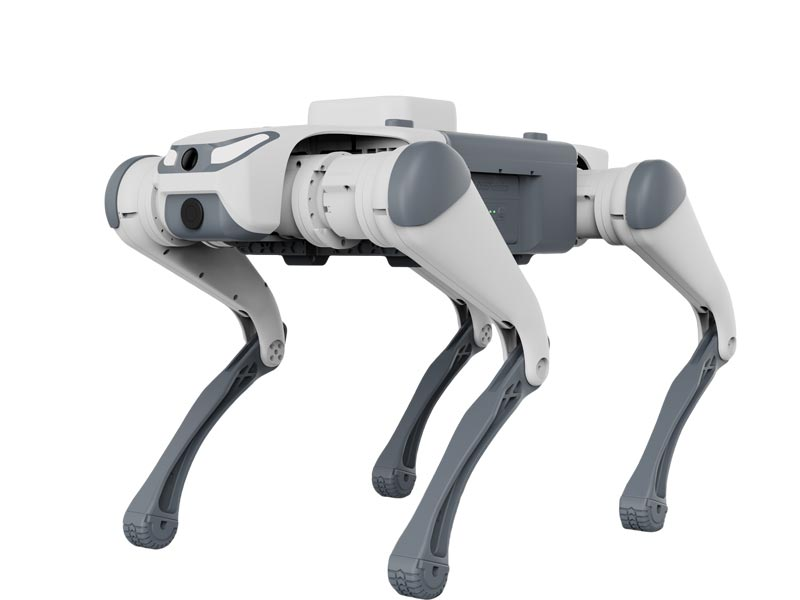
\includegraphics[scale=0.25]{gambar/quadruped_robot.jpg}
  \caption{DeepRobotics Lite3}
  \label{fig:quadruped_robot}
\end{figure}

Dalam hal desain dan kontrol, robot \emph{quadruped} mengadopsi prinsip-prinsip biomekanika
untuk meniru pola gerak alami hewan. Pola gerak ini, yang dikenal sebagai \emph{gait},
mencakup berbagai cara berjalan seperti \emph{trot}, \emph{pace}, dan \emph{gallop},
yang masing-masing digunakan tergantung pada kecepatan dan kondisi medan.
Implementasi gerakan ini membutuhkan sistem kendali yang kompleks,
termasuk algoritma keseimbangan dinamis dan kontrol koordinasi antar kaki.
Beberapa robot \emph{quadruped} menggunakan sensor inersia (IMU), kamera,
serta teknologi kecerdasan buatan (AI) untuk meningkatkan kesadaran situasional dan kemampuan navigasi secara otonom.

Robot \emph{quadruped} dapat dikategorikan berdasarkan sistem aktuasi yang digunakan,
yaitu robot dengan aktuasi elektrik, hidraulik, atau kombinasi keduanya.
Robot dengan aktuator elektrik cenderung lebih ringan dan lebih efisien dalam hal konsumsi daya,
sementara robot hidraulik lebih kuat dan mampu menangani beban yang lebih berat.
Beberapa robot \emph{quadruped} yang telah dikembangkan termasuk Spot dari Boston Dynamics,
ANYmal dari ANYbotics, dan Unitree Go1, yang digunakan dalam berbagai penelitian dan aplikasi industri.

Penggunaan robot \emph{quadruped} terus berkembang, terutama dalam bidang militer, eksplorasi luar angkasa,
pertanian, dan robotika layanan. Dengan kemampuannya untuk bergerak secara fleksibel di medan yang menantang
dan membawa beban tambahan, robot ini memiliki potensi besar untuk digunakan dalam
skenario di mana robot beroda atau berkaki dua mengalami kesulitan.
Tantangan utama dalam pengembangan robot \emph{quadruped} meliputi efisiensi energi, ketahanan perangkat keras,
dan peningkatan kecerdasan buatan agar mampu beradaptasi lebih baik dengan lingkungan yang tidak terstruktur.

\subsection{Robot Lengan}

\begin{figure} [H] \centering
  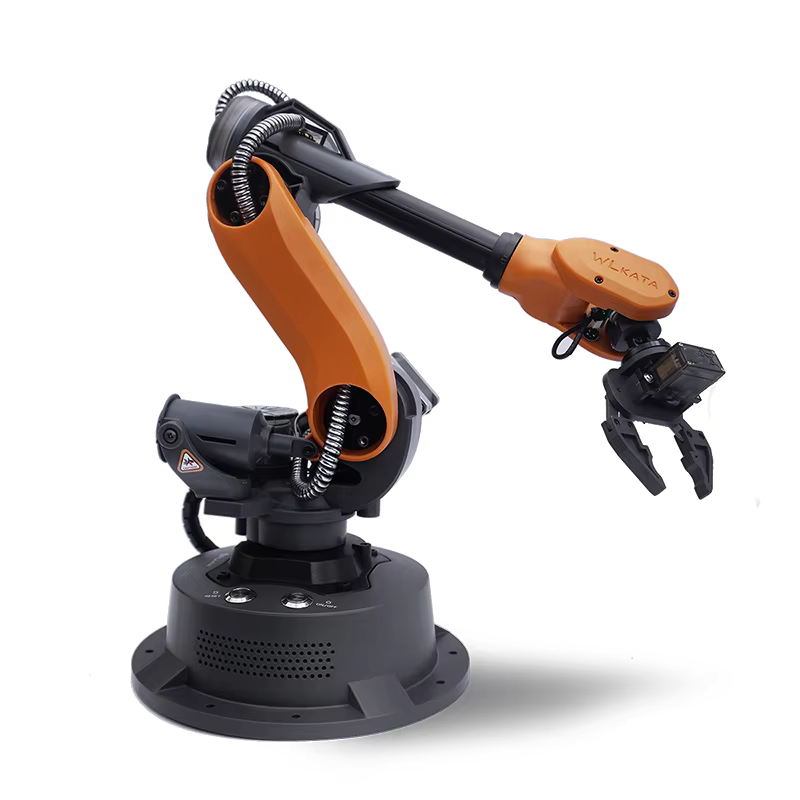
\includegraphics[scale=0.25]{gambar/arm_robot.png}
  \caption{Salah Satu Jenis Robot Lengan Dari Wlkata}
  \label{fig:arm_robot}
\end{figure}
Robot lengan, atau \emph{robotic arm}, adalah jenis robot yang dirancang untuk meniru fungsi lengan manusia
dalam melakukan berbagai tugas manipulasi objek. Robot ini umumnya terdiri dari serangkaian sambungan (\emph{joints})
dan batang (\emph{links}) yang memungkinkan pergerakan fleksibel dalam berbagai arah. Dengan kombinasi aktuator,
sensor, dan sistem kendali yang kompleks, robot lengan mampu melakukan tugas-tugas seperti \emph{pick-and-place},
perakitan, pengelasan, pengecatan, serta tugas presisi lainnya dalam industri manufaktur, medis, dan penelitian.

Robot lengan dapat dikategorikan berdasarkan konfigurasi kinematiknya, seperti robot kartesian,
robot SCARA (\emph{Selective Compliance Articulated Robot Arm}), robot artikulasi, dan robot delta.
Robot kartesian memiliki tiga derajat kebebasan dalam sumbu X, Y, dan Z, serta sering digunakan
dalam aplikasi yang membutuhkan pergerakan linier, seperti mesin CNC. Robot SCARA memiliki fleksibilitas
lebih dalam bidang horizontal dan umumnya digunakan dalam proses perakitan cepat. Robot artikulasi,
yang memiliki sambungan berputar serupa dengan lengan manusia, digunakan dalam berbagai aplikasi industri
dan medis karena kemampuannya untuk mencapai berbagai sudut dan melakukan gerakan yang kompleks.
Sementara itu, robot delta, yang memiliki struktur paralel, biasanya diterapkan dalam industri makanan
dan farmasi untuk tugas-tugas kecepatan tinggi dengan presisi tinggi.

Dalam implementasi teknologinya, robot lengan menggunakan berbagai sensor dan aktuator untuk
meningkatkan akurasi dan efisiensi operasional\parencite{ZhenXie_lbrgar}. Sensor posisi dan kecepatan digunakan untuk
mengontrol gerakan sendi, sementara sensor gaya dan torsi memungkinkan robot berinteraksi
dengan lingkungan secara lebih presisi, misalnya dalam tugas perakitan yang membutuhkan kepekaan
terhadap perubahan gaya. Kamera dan sistem visi komputer juga sering digunakan untuk mendeteksi
dan mengenali objek, memungkinkan robot melakukan tugas-tugas berbasis kecerdasan buatan
seperti penyortiran otomatis dan inspeksi kualitas produk.

Sistem kendali robot lengan dapat dibagi menjadi kontrol terbuka (\emph{open-loop control}) dan
kontrol tertutup (\emph{closed-loop control}). Dalam sistem kontrol terbuka, perintah gerakan diberikan
tanpa umpan balik dari sensor, sementara dalam kontrol tertutup, sistem terus memantau dan
menyesuaikan gerakan berdasarkan informasi dari sensor, sehingga menghasilkan pergerakan
yang lebih akurat dan adaptif. Algoritma kendali seperti \emph{PID control}, \emph{inverse kinematics},
dan \emph{reinforcement learning} sering digunakan untuk meningkatkan performa robot dalam
menyesuaikan gerakan terhadap tugas tertentu.

Robot lengan telah menjadi bagian penting dalam revolusi industri dan otomatisasi modern.
Dalam industri manufaktur, robot ini digunakan untuk meningkatkan produktivitas dan
mengurangi risiko cedera pada pekerja manusia. Di bidang medis, robot bedah seperti
da Vinci Surgical System memungkinkan prosedur bedah yang lebih presisi dan minim invasif.
Selain itu, dalam dunia penelitian dan eksplorasi luar angkasa, robot lengan digunakan
dalam eksperimen ilmiah dan misi eksplorasi, seperti lengan robotik yang dipasang pada \emph{rover} penjelajah Mars.

\subsection{Human-Robot Interaction}

Interaksi manusia-robot (\emph{Human-Robot Interaction}) adalah bidang multidisiplin yang berfokus
pada cara manusia dan robot berkomunikasi, bekerja sama, serta berbagi lingkungan dalam berbagai konteks aplikasi.
Dengan semakin berkembangnya teknologi robotika, interaksi antara manusia dan robot tidak lagi
terbatas pada pengoperasian manual di lingkungan industri, tetapi juga meluas ke bidang kesehatan, layanan pelanggan,
edukasi, hingga penggunaan dalam kehidupan sehari-hari. Oleh karena itu, desain dan pengembangan sistem interaksi yang intuitif,
aman, serta efisien menjadi aspek yang sangat penting dalam penelitian dan implementasi robotika modern.

HRI dapat dikategorikan berdasarkan tingkat keterlibatan manusia dalam pengendalian robot, yaitu \emph{remote interaction},
\emph{supervisory control}, \emph{collaborative interaction}, dan \emph{fully autonomous interaction}. Dalam \emph{remote interaction}, manusia
mengendalikan robot dari jarak jauh, misalnya dalam operasi militer atau eksplorasi luar angkasa. Pada \emph{supervisory control},
manusia memberikan instruksi tingkat tinggi sementara robot mengeksekusi tugasnya secara semi-otomatis, seperti dalam sistem
robot bedah atau kendaraan otonom. Dalam \emph{collaborative interaction}, manusia dan robot bekerja berdampingan, seperti di pabrik
manufaktur yang menerapkan cobots (\emph{collaborative robots}). Sementara itu, dalam \emph{fully autonomous interaction}, robot dapat
beroperasi secara mandiri dengan pemahaman penuh terhadap lingkungan dan kebutuhan manusia, seperti asisten rumah tangga
berbasis kecerdasan buatan.

\begin{figure} [H] \centering
    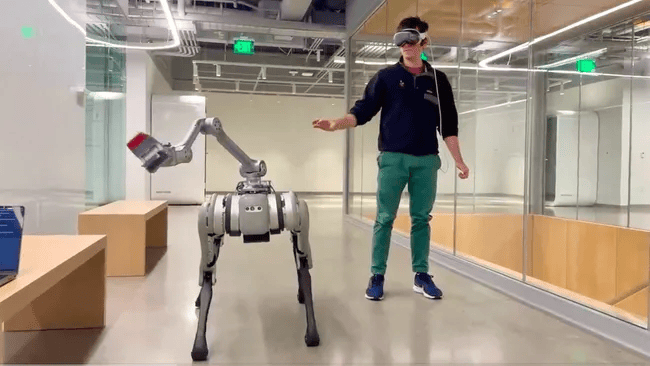
\includegraphics[scale=0.4]{gambar/HRI daster.png}
    \caption{Salah Satu Bentuk Interaksi Supervisory Control\parencite{img_HRI}}
    \label{fig:HRI_daster}
\end{figure}

Salah satu tantangan utama dalam HRI adalah pengembangan sistem komunikasi yang efektif antara manusia dan robot\parencite{QifanZhang_tlihrifamoagdwqr}.
Metode komunikasi ini bisa berupa antarmuka fisik seperti tombol dan \emph{joystick}, antarmuka berbasis suara (\emph{speech recognition}),
bahasa tubuh, serta ekspresi wajah yang dapat dikenali oleh robot menggunakan sistem visi komputer. Dalam beberapa sistem,
robot dapat memahami emosi manusia dengan mendeteksi ekspresi wajah dan intonasi suara, memungkinkan interaksi yang lebih alami dan
intuitif. Sebagai contoh, robot sosial seperti Pepper dan NAO dirancang untuk memahami dan merespons interaksi manusia dengan cara
yang lebih mirip interaksi antarmanusia. Keamanan dan kepercayaan juga menjadi faktor krusial dalam interaksi manusia-robot,
terutama dalam lingkungan di mana robot bekerja berdampingan dengan manusia. Penggunaan sensor dan algoritma kecerdasan buatan
memungkinkan robot untuk mengenali dan merespons keberadaan manusia di sekitarnya secara aman. Misalnya, robot kolaboratif yang
digunakan dalam industri manufaktur sering kali dilengkapi dengan sensor gaya dan torsi untuk mendeteksi adanya hambatan fisik,
sehingga dapat memperlambat atau menghentikan gerakan ketika mendekati manusia. Selain itu, desain robot yang lebih ramah secara
visual dan ergonomis dapat meningkatkan kepercayaan pengguna terhadap teknologi ini.  

\begin{figure} [H] \centering
    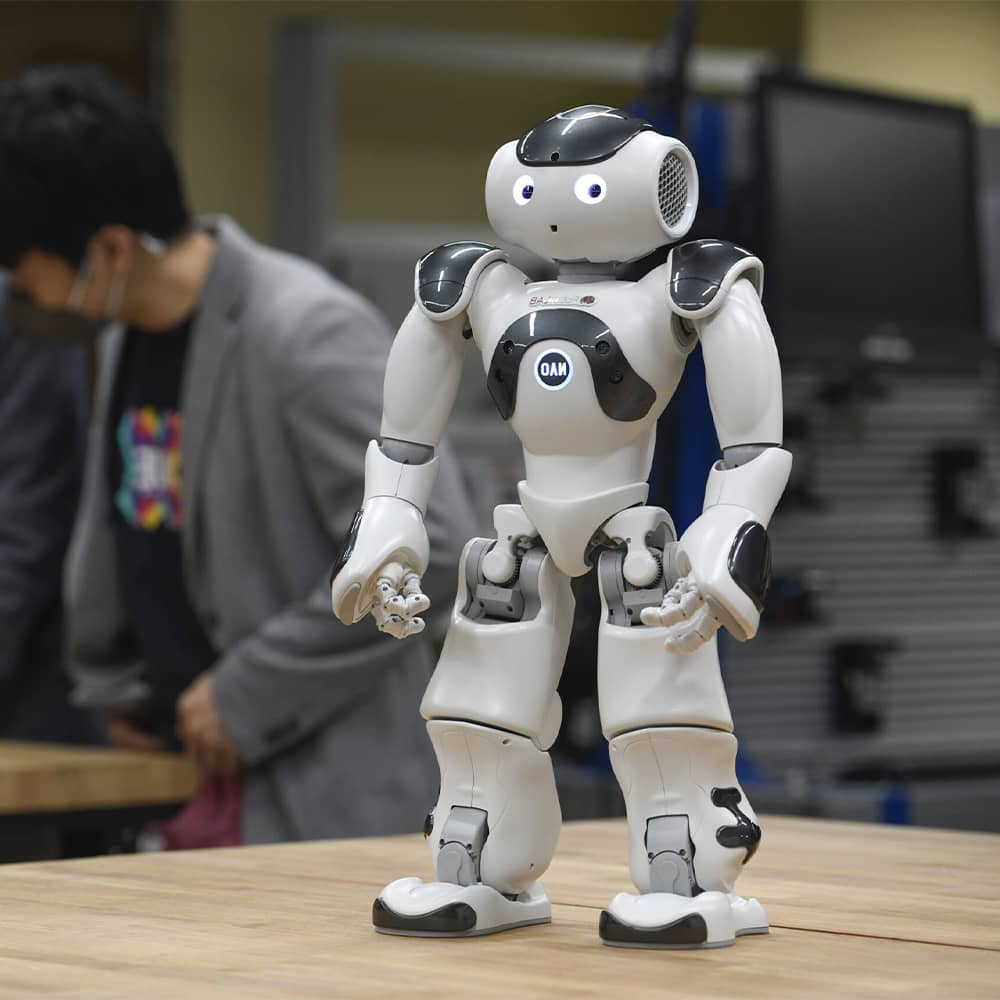
\includegraphics[scale=0.2]{gambar/NAO_robot.jpg}
    \caption{Salah Satu Contoh Robot Sosial NAO}
    \label{fig:HRI_NAO_daster}
\end{figure}

Dalam bidang kesehatan, HRI memainkan peran penting dalam pengembangan robot pendamping bagi lansia atau pasien dengan kebutuhan khusus.
Robot semacam ini dapat membantu dalam aktivitas sehari-hari, memberikan pengingat untuk minum obat, atau bahkan menyediakan interaksi
sosial bagi pengguna yang mengalami kesepian. Selain itu, dalam terapi anak-anak dengan autisme, robot telah digunakan untuk membantu
meningkatkan keterampilan sosial mereka dengan interaksi yang lebih konsisten dan dapat diprediksi dibandingkan dengan manusia.  
Seiring dengan meningkatnya penggunaan robot dalam berbagai aspek kehidupan, tantangan etika dalam HRI juga menjadi perhatian utama.
Isu-isu seperti privasi data pengguna, pengaruh robot terhadap tenaga kerja manusia, serta batasan dalam interaksi emosional antara
manusia dan robot menjadi bahan diskusi yang terus berkembang.

\subsection{Grasping Pose Detection}

\emph{Grasping pose detection} adalah bidang yang berfokus pada pengenalan dan
penentuan posisi optimal bagi robot untuk mengambil, memegang, dan memanipulasi objek dengan tangannya atau
\emph{end-effector}. \emph{Grasping pose detection} merupakan aspek krusial dalam sistem robotik, terutama
pada aplikasi seperti otomatisasi industri, layanan rumah tangga, logistik, serta bidang kesehatan. Kemampuan
robot untuk secara akurat menentukan bagaimana cara menggenggam suatu objek sangat bergantung pada berbagai
faktor seperti bentuk, ukuran, tekstur, dan material dari objek tersebut, serta kondisi lingkungan sekitarnya\parencite{ZhenXie_lbrgar}.

\emph{Grasping pose detection} sering kali mengandalkan kombinasi antara teknologi sensor, algoritma, serta kecerdasan buatan.
Sensor yang umum digunakan meliputi kamera RGB, kamera \emph{depth}, sensor LiDAR, dan sensor sentuh (\emph{tactile sensor}).
Kamera RGB-D, seperti Intel RealSense atau Microsoft Kinect, memungkinkan robot untuk menangkap informasi visual serta kedalaman objek,
sehingga dapat memahami bentuk tiga dimensi dari objek yang akan digenggam. Sementara itu, sensor sentuh memberikan umpan balik langsung
tentang tekanan dan gesekan yang diterapkan oleh gripper robot terhadap objek yang dipegang, memungkinkan penyesuaian genggaman secara
\emph{real-time} untuk menghindari tergelincir atau merusak objek.
Algoritma yang digunakan dalam \emph{Grasping Pose Detection} umumnya memanfaatkan teknik pengolahan citra dan pembelajaran mesin.
Pendekatan berbasis visi komputer sering kali menggunakan teknik seperti \emph{edge detection}, \emph{feature extraction}, dan segmentasi objek
untuk mengidentifikasi kontur serta titik-titik kritis pada objek. Dengan kemajuan kecerdasan buatan, terutama \emph{deep learning}, banyak
penelitian telah mengembangkan model berbasis jaringan saraf konvolusional (\emph{Convolutional Neural Networks} atau CNN) serta model
berbasis \emph{Reinforcement Learning} untuk mempelajari strategi genggaman yang lebih fleksibel dan adaptif.
Selanjutnya, metode berbasis \emph{motion planning} digunakan untuk membantu robot lengan dalam
merancang lintasan yang optimal sehingga robot dapat mencapai posisi genggaman tanpa menabrak rintangan di sekitarnya.
Metode ini sering dikombinasikan dengan pendekatan berbasis \emph{inverse kinematics} untuk menghitung konfigurasi sendi yang
memungkinkan robot mencapai target genggaman dengan sudut dan orientasi yang sesuai.

\begin{figure} [H] \centering
    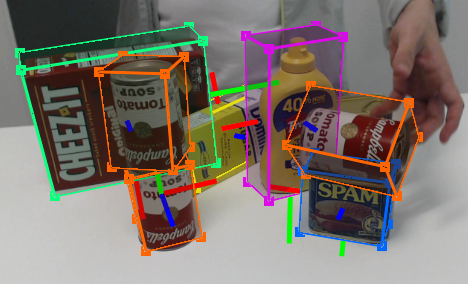
\includegraphics[scale=0.95]{gambar/grasping_pose_detection.png}
    \caption{Hasil Riset NVIDIA dalam pemanfaatan deep learning untuk grasping robot\parencite{img_grasping_daster}}
    \label{fig:grasping_daster}
\end{figure}

Salah satu tantangan utama dalam \emph{Grasping Pose Detection} adalah menghadapi objek dengan bentuk yang kompleks,
permukaan yang reflektif, atau kondisi pencahayaan yang berubah-ubah. Selain itu, keberadaan lingkungan yang dinamis,
seperti objek yang bergerak atau berubah posisinya, juga menambah kompleksitas dalam menentukan strategi genggaman
yang optimal.
Dalam aplikasi nyata, \emph{Grasping Pose Detection} telah digunakan dalam berbagai bidang,
seperti robot pemindah barang di gudang \emph{e-commerce}, sistem asisten robotik di rumah tangga,
hingga robot medis yang dapat memegang dan memanipulasi peralatan bedah dengan presisi tinggi.

\subsection{Pengolahan Citra}
Dalam suatu sistem komputasi, citra yang ditemui pada dunia nyata tidak dapat secara
langsung direpresentasikan oleh komputer. Dalam merubah bentuk citra di dunia nyata atau
yang sering disebut citra analog perlu dilakukan perubahan dengan menggunakan sistem \emph{sampling}.
Sistem \emph{sampling} ini berguna untuk mengubah citra analog menjadi M baris N kolom dan
hasil ini dapat didefinisikan sebagai citra diskrit. Pertemuan titik antara M baris dan N kolom
ini dinamakan dengan Piksel atau titik terkecil dari sebuah citra digital. Selain sistem \emph{sampling},
di dalam citra digital juga terdapat kuantisasi. Kuantitasi adalah sebuah pemberian nilai-nilai
tertentu pada sebuah piksel di dalam citra digital. Nilai kuantisasi ini dapat merepresentasikan
warna maupun kecerahan dari piksel di dalam sebuah citra digital.

Dengan adanya piksel dan hasil nilai kuantisasi maka dapat dilakukan pengoperasian matematika pada nilai kuantisasi
di seluruh piksel yang dimiliki sebuah citra digital. Salah satu cara pengolahan yang paling mudah adalah dengan
menggunakan \emph{library} yang bernama OpenCV\parencite{RDKusumanto_pcdumompwmnr}. OpenCV mampu membantu dalam pemrosesan
data nilai suatu gambar yang dimana di dalam komputer hasil dari \emph{sampling} dan kuantisasi ini direpresentasikan
sebagai sebuah \emph{array}. Pengolahan citra sering digunakan untuk mempersiapakan gambar sebelum diolah oleh program
\emph{machine learning} sehingga menghasilkan hasil keputusan yang jauh lebih baik dibandingkan langsung memberikan gambar.

Pengolahan citra memainkan peran penting dalam operasi robot lengan, terutama dalam meningkatkan akurasi
dan efisiensi manipulasi objek dalam berbagai lingkungan. Dengan menggunakan kamera sebagai sensor visual, robot lengan
dapat memperoleh informasi mengenai posisi, orientasi, serta karakteristik objek yang akan dipegang atau dipindahkan.
Teknologi pengolahan citra memungkinkan robot untuk mendeteksi dan mengenali objek, mengklasifikasikan bentuk dan warna,
serta menyesuaikan gerakan lengan agar sesuai dengan kondisi lingkungan.

\subsection{ROS}
\emph{Robot Operating System} (ROS) adalah sebuah \emph{framework open-source} yang dirancang untuk mendukung pengembangan
perangkat lunak robotika yang kompleks dan modular. Meskipun namanya mengandung kata "\emph{Operating System}," ROS
sebenarnya bukanlah sistem operasi yang independen, melainkan sebuah \emph{middleware} yang berjalan di atas sistem operasi
seperti Ubuntu (Linux) dan menyediakan berbagai \emph{tools} serta \emph{library} untuk membantu \emph{developer} dalam membangun
aplikasi robotika. ROS dikembangkan oleh Willow Garage dan sejak itu telah berkembang menjadi standar industri
dalam komunitas robotika, baik dalam lingkungan akademik maupun industri.

\begin{figure} [H] \centering
    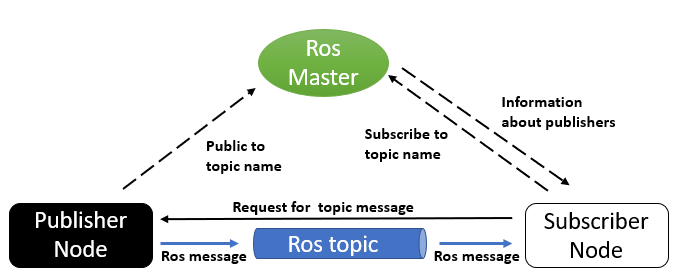
\includegraphics[scale=0.65]{gambar/ros_system.png}
    \caption{Sistem Kerja ROS\parencite{img_ros_system}}
    \label{fig:ros_system}
\end{figure}

Salah satu keunggulan utama ROS adalah arsitektur berbasis \emph{node} dan komunikasi antarproses\parencite{ros_website}. Dalam ROS,
sebuah sistem robot dapat dibagi menjadi beberapa \emph{node}, di mana setiap \emph{node} bertanggung jawab untuk menjalankan tugas
tertentu, seperti pemrosesan sensor, kendali aktuator, atau perencanaan gerak. tiap-tiap \emph{node} ini dapat berkomunikasi
satu sama lain menggunakan ROS \emph{topics}, \emph{services}, dan \emph{actions}, yang memungkinkan sistem menjadi lebih modular dan
fleksibel. Misalnya, sebuah \emph{mobile robot} yang menggunakan kamera dan LIDAR untuk navigasi dapat memiliki satu \emph{node}
untuk pemrosesan citra, satu \emph{node} untuk pemetaan lingkungan, dan satu \emph{node} untuk pengendalian gerak, yang semuanya
bekerja secara terpisah tetapi tetap dapat saling bertukar informasi.
Salah satu fitur penting lain dalam ROS adalah dukungan terhadap sistem terdistribusi, yang memungkinkan
beberapa komputer untuk bekerja secara bersama-sama dalam satu jaringan ROS. Hal ini sangat berguna dalam
sistem robotik yang kompleks, misalnya pada robot otonom yang terdiri dari beberapa subsistem terpisah
seperti robot lengan yang bekerja bersama dengan \emph{mobile robot}.

Selain itu, ROS menyediakan berbagai \emph{library} yang telah dioptimalkan untuk pemrosesan sensor,
SLAM (\emph{Simultaneous Localization and Mapping}), perencanaan gerak, kontrol robotik, dan visi komputer.
Salah satu \emph{library} yang sering digunakan dalam ROS adalah MoveIt!, yang mendukung perencanaan gerak
pada robot manipulator seperti lengan robot. Selain itu, ada juga \emph{library} seperti OpenCV untuk
pemrosesan citra, PCL untuk pemrosesan data 3D dari LIDAR, serta integrasi dengan
berbagai jenis sensor dan aktuator melalui \emph{driver} yang telah dikembangkan dalam komunitas ROS.
ROS juga mendukung simulasi robot melalui integrasi dengan Gazebo, RViz, dan simulasi berbasis \emph{physics engine} lainnya.
Gazebo memungkinkan \emph{developer} untuk menguji algoritma kontrol robot dalam lingkungan simulasi sebelum diterapkan pada
perangkat keras nyata, yang sangat berguna untuk menghindari kerusakan pada robot akibat kesalahan pemrograman. RViz,
di sisi lain, adalah alat visualisasi yang digunakan untuk menampilkan data sensor, trajektori robot, serta hasil dari
berbagai algoritma pemrosesan yang berjalan di dalam sistem ROS.

\subsection{QT}

Qt adalah sebuah framework pengembangan perangkat lunak yang bersifat \emph{open-source} dan komersial,
yang digunakan untuk membangun aplikasi dengan antarmuka grafis (GUI) serta aplikasi berbasis
embedded system dan IoT. Qt menyediakan berbagai \emph{library} dan \emph{tools}
yang memungkinkan pengembang untuk membuat aplikasi lintas \emph{platform} yang dapat berjalan pada berbagai
sistem operasi seperti Windows, macOS, Linux, serta perangkat mobile seperti Android dan iOS.
Salah satu keunggulan utama Qt adalah penggunaan bahasa pemrograman C++ dengan dukungan dari sistem
\emph{meta-object} dan \emph{signal-slot} yang memungkinkan komunikasi antar objek dalam arsitektur \emph{event-driven}.
Selain itu, Qt juga mendukung pemrograman menggunakan Qt Quick dan Qt Modeling Language,
yang memudahkan pengembangan antarmuka grafis yang dinamis dan responsif dengan pendekatan berbasis deklaratif. 

Dalam pengembangannya, Qt menyediakan berbagai modul yang mencakup aspek fundamental seperti
tampilan GUI, jaringan, pemrosesan multimedia, hingga integrasi dengan sistem robotika melalui ROS. Dengan fitur-fitur ini,
Qt sering digunakan dalam berbagai bidang, mulai dari aplikasi desktop, sistem otomasi industri,
perangkat medis, hingga sistem kendali robot. Qt juga memiliki keunggulan dalam optimalisasi kinerja
melalui sistem \emph{rendering} berbasis OpenGL dan Vulkan, sehingga cocok untuk aplikasi yang membutuhkan
visualisasi grafis tinggi. Dalam penelitian ini, Qt digunakan sebagai \emph{platform} utama dalam pengembangan
GUI untuk sistem interaksi manusia-robot, di mana operator dapat memilih
objek yang akan diambil oleh robot melalui antarmuka visual yang intuitif. Dengan fleksibilitas dan
performa tinggi yang ditawarkan oleh Qt, sistem GUI dapat berjalan dengan responsif dan dapat diintegrasikan
dengan berbagai sensor serta perangkat keras yang mendukung robotika. Qt juga mendukung pengembangan modular
dengan konsep \emph{Model-View-Controller} (MVC), sehingga memudahkan dalam pemeliharaan dan pengembangan sistem
yang lebih kompleks.
  \cleardoublepage

  % Konten metodologi
  \chapter{METODOLOGI}

% Ubah konten-konten berikut sesuai dengan isi dari metodologi

\section{Bahan dan peralatan yang digunakan}

Peralatan yang digunakan untuk penelitian ini antara lain:

\begin{enumerate}
  \item \textbf{GraspNet}, digunakan sebagai \emph{framework} robot lengan untuk
  melakukan tugas berupa \emph{autonomous grasping}. GraspNet sendiri adalah sebuah \emph{framework}
  berbasis \emph{deep learning} yang dirancang untuk melakukan prediksi \emph{pose grasping} secara akurat bagi lengan robot.
  \item \textbf{ROS}, yang mana merupakan sebuah \emph{framework}
  \emph{open-source} yang menyediakan kumpulan \emph{software}, \emph{library}, dan \emph{tools} untuk membantu pengembangan,
  pengendalian, serta komunikasi antar komponen dalam sistem robotik secara modular dan terdistribusi.
  \item \textbf{QT}, merupakan \emph{framework} pengembangan aplikasi \emph{cross-platform} yang berbasis C++,
  digunakan untuk membangun antarmuka grafis (GUI) dan aplikasi dengan performa tinggi serta kompatibilitas luas di berbagai sistem operasi.
  \item \textbf{Hardware}, Hardware yang digunakan dalam penelitian ini adalah robot \emph{quadruped} dari DeepRobotics,
  robot lengan dengan servo motor dynamixel, serta kontroler custom yang dikembangkan oleh tim robot Ichiro ITS.
\end{enumerate}

% \lipsum[11]
% % Contoh input gambar dengan format *.jpg
% \begin{figure} [H] \centering
%   % Nama dari file gambar yang diinputkan
%   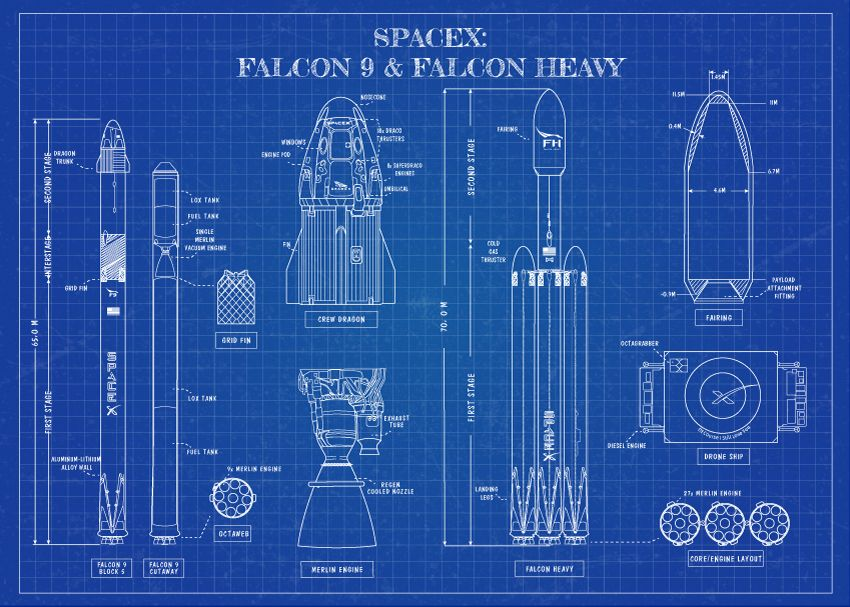
\includegraphics[scale=0.45]{gambar/blueprint.jpg}
%   % Keterangan gambar yang diinputkan
%   \caption{\emph{Blueprint} roket yang akan diuji coba \parencite{SpaceXBlueprint}}
%   % Label referensi dari gambar yang diinputkan
%   \label{fig:Blueprint}
% \end{figure}
% % Contoh penggunaan referensi dari gambar yang diinputkan
% Pada \emph{blueprint} yang tertera di Gambar \ref{fig:Blueprint}. \lipsum[12]

\section{Metode yang digunakan}

Metodologi yang digunakan pada penelitian ini terdiri dari beberapa tahapan seperti yang
ditunjukkan pada gambar berikut.

\begin{figure} [H] \centering
  % Nama dari file gambar yang diinputkan
  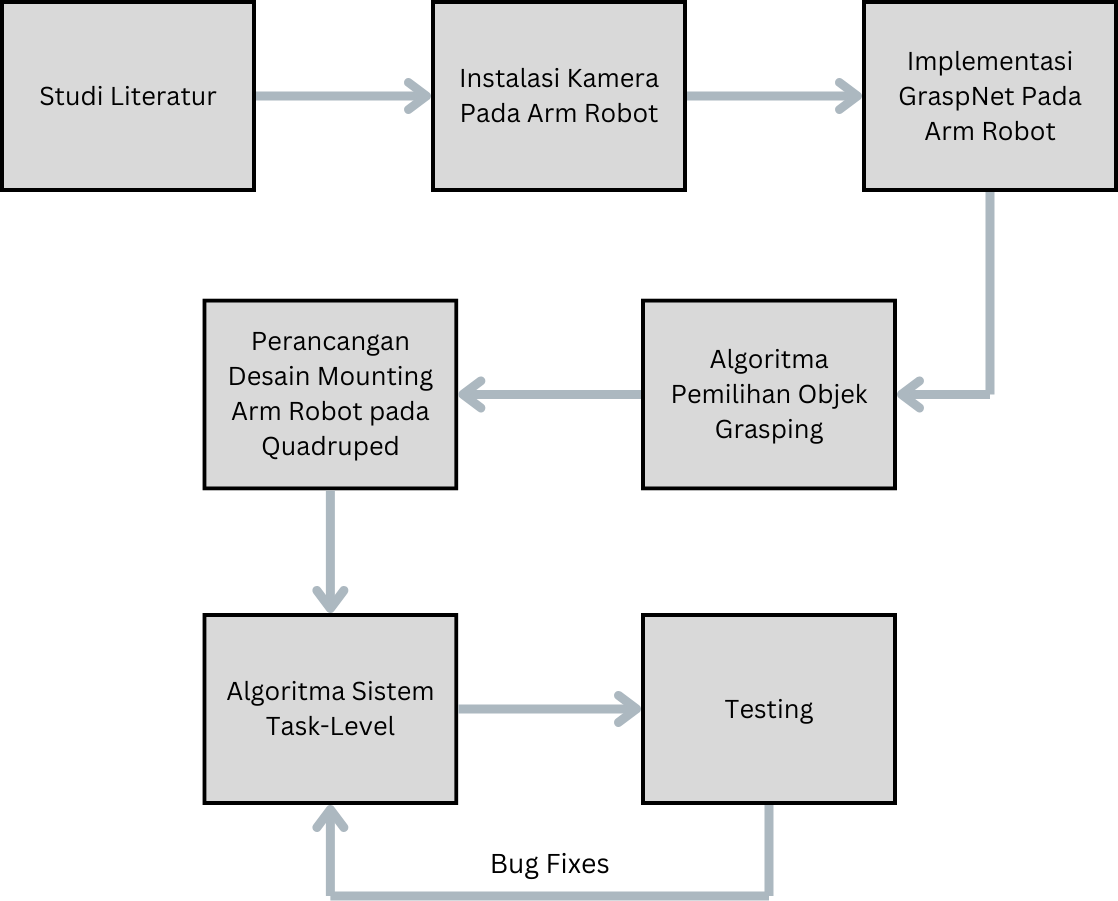
\includegraphics[scale=0.4]{gambar/Blok Diagram Metodologi.png}
  % Keterangan gambar yang diinputkan
  \caption{Blok Diagram Perancangan Penelitian}
  % Label referensi dari gambar yang diinputkan
  \label{fig:diagram_metode}
\end{figure}

Berikut merupakan penjelasan dari tiap tahapan pada metode penelitian di atas :
\begin{enumerate}
  \item \textbf{Studi Literatur} : Tahap awal dalam penelitian ini adalah melakukan studi literatur untuk memahami konsep
  dan teknologi yang mendasari penelitian. Studi literatur dilakukan terhadap berbagai sumber
  seperti jurnal ilmiah, buku referensi, dan publikasi konferensi yang membahas topik terkait,
  seperti robot lengan (\emph{robotic arm}), robot \emph{quadruped}, GraspNet, algoritma \emph{grasping}, serta
  integrasi sensor dan sistem kendali. Penelitian sebelumnya yang relevan akan dikaji untuk
  memahami pendekatan yang telah dilakukan dan menemukan potensi perbaikan atau inovasi
  yang dapat diterapkan dalam penelitian ini. Literatur terkait metode pemasangan kamera
  untuk persepsi visual pada robot lengan juga dikaji untuk memilih konfigurasi sensor yang optimal.

  \item \textbf{Instalasi Kamera Pada Robot Lengan} : Tahap ini bertujuan untuk mengintegrasikan
  sistem persepsi visual menggunakan kamera pada robot lengan. Kamera akan dipasang di posisi
  yang memungkinkan robot melihat objek yang akan diambil, yaitu di pangkal bagian \emph{gripper}.
  \begin{figure} [H] \centering
    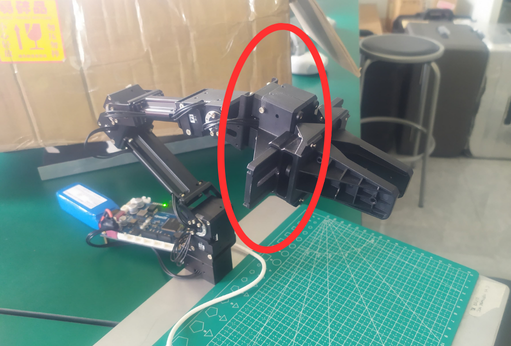
\includegraphics[scale=0.5]{gambar/penempatan kamera.png}
    \caption{Lokasi Kamera}
    \label{fig:lokasi_kamera}
  \end{figure}
  Posisi ini dipilih karena memungkinkan untuk robot dapat mengontrol sudut yang dilihat oleh kamera.
  Proses pemasangan menggunakan mounting yang didesain dan dicetak menggunakan \emph{3D Printer}
  
  \item \textbf{Implementasi GraspNet Pada Robot Lengan} : Pada tahap ini, algoritma GraspNet
  akan diimplementasikan untuk mendeteksi \emph{pose} optimal dalam proses \emph{grasping}.
  GraspNet merupakan model berbasis \emph{machine learning} yang mampu memprediksi berbagai
  kemungkinan posisi dan orientasi tangan robot dalam mencengkeram suatu objek.
  \begin{figure} [H] \centering
    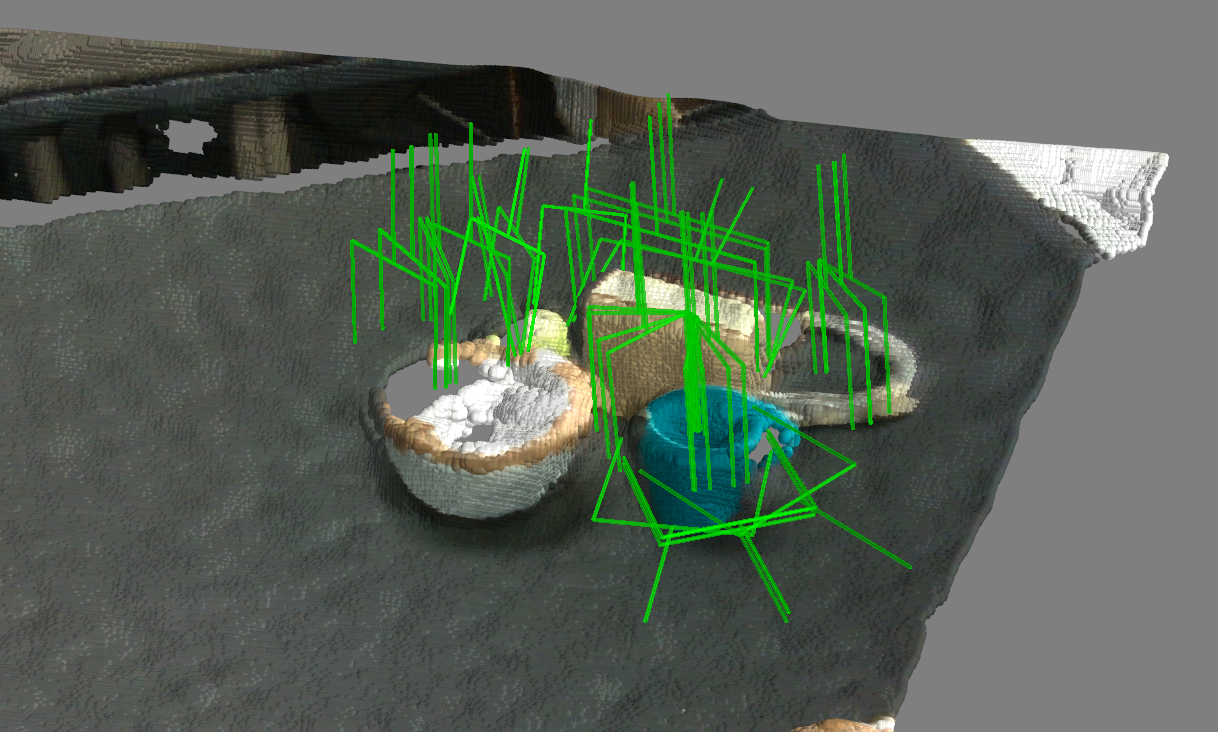
\includegraphics[scale=0.15]{gambar/contoh_hasil_graspdetect.png}
    \caption{Contoh hasil dari grasp detection\parencite{img_result_graspdetect}}
    \label{fig:graspdetect result}
  \end{figure}
  Model GraspNet akan diterapkan pada data citra yang diperoleh dari kamera, sehingga sistem dapat menentukan
  titik \emph{grasping} terbaik dengan mempertimbangkan faktor seperti bentuk, orientasi, dan jenis objek.
  Terdapat dua jenis citra yang digunakan dalam model GraspNet, yaitu \emph{rgb frame} dan \emph{depth frame}.
  \begin{figure} [H] \centering
    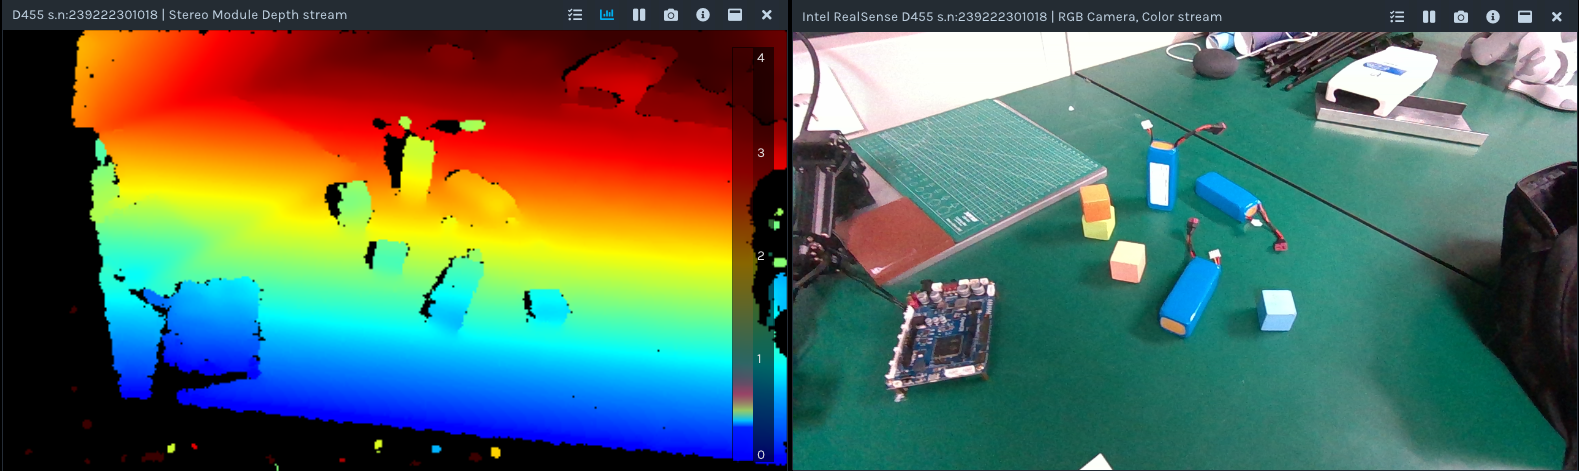
\includegraphics[scale=0.3]{gambar/depth_rgb.png}
    \caption{Perbandingan depth dengan rgb}
    \label{fig:depth_rgb}
  \end{figure}
  \emph{Rgb frame} berperan dalam memberikan informasi visual seperti warna, tekstur, dan bentuk objek
  untuk membantu segmentasi dan identifikasi. Sedangkan \emph{depth frame} berperan dalam menyediakan
  informasi kedalaman dan struktur 3D objek untuk menentukan posisi dan orientasi grasping yang optimal.
  Pengujian awal dilakukan untuk menilai performa algoritma dalam mendeteksi \emph{pose} \emph{grasping}
  pada berbagai jenis objek. Jika diperlukan, model GraspNet dapat disesuaikan atau
  di-\emph{fine-tune} untuk meningkatkan akurasi dan efisiensi sistem.
  
  \item \textbf{Algoritma Pemilihan Objek Grasping} : Pemilihan objek yang akan di-\emph{grasp} dilakukan
  oleh operator (manusia) melalui antarmuka interaktif, sehingga menghilangkan kemungkinan kesalahan
  keputusan robot dalam melakukan pemilihan objek.
  \begin{figure} [H] \centering
    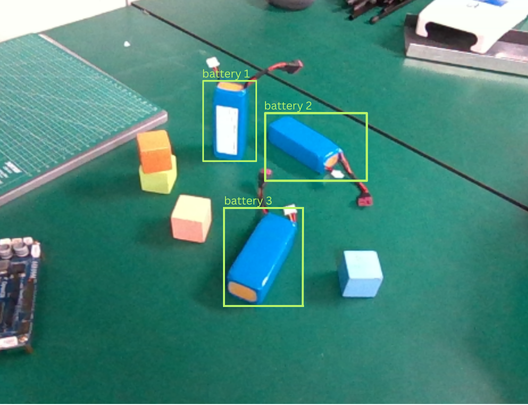
\includegraphics[scale=0.5]{gambar/pemilihan objek.png}
    \caption{Ilustrasi Tampilan Saat Proses Pemilihan Objek}
    \label{fig:pemilihan_objek}
  \end{figure}
  Bounding box akan ditampilkan pada objek yang terdeteksi
  melalui kamera, sehingga membiarkan operator memilih objek tersebut melalui klik pada GUI. Setelah operator
  memilih objek, sistem akan menjalankan GraspNet untuk menentukan titik optimal grasping dan
  mengeksekusi perintah tersebut pada robot lengan. Fitur konfirmasi dan pemberian indikator pada objek
  juga ditambahkan agar interaksi lebih intuitif.

  \item \textbf{Perancangan Desain Mounting Robot Lengan Pada Quadruped} : Salah satu tantangan utama dalam penelitian
  ini adalah integrasi robot lengan dengan platform \emph{quadruped}. Desain mounting harus mempertimbangkan faktor-faktor
  seperti keseimbangan, distribusi beban, dan fleksibilitas gerakan. Perancangan dilakukan menggunakan perangkat lunak CAD
  seperti Fusion 360 untuk memastikan desain yang optimal. Proses pemasangan dilakukan dengan memastikan bahwa robot
  \emph{quadruped} tetap dapat bergerak dengan stabil meskipun membawa robot lengan.

  \item \textbf{Algoritma Sistem Task-Level} : Setelah integrasi perangkat keras selesai, tahap selanjutnya adalah
  mengembangkan algoritma \emph{task-level} yang mengoordinasikan gerakan robot lengan dan robot \emph{quadruped}.
  Algoritma ini mengatur bagaimana robot menyelesaikan tugas-tugas seperti mendekati objek, mengambilnya, dan
  membawanya ke lokasi yang diinginkan. Jadi nantinya dalam menjalankan tugas, robot memiliki urutan level terkait aksi yang akan dilakukannya.
  Misalnya di level pertama, robot ditentukan oleh operator untuk akan menuju ke ruangan mana. 
  Lalu level berikutnya, robot menuju ke bagian tertentu di ruangan tersebut. Lalu ada level dimana ditentukan objek mana yang akan di ambil.
  Hingga tujuan mana yang akan dituju oleh robot setelah mengambil barang. Selain itu,
   Sistem ini juga harus mempertimbangkan faktor lingkungan, seperti menghindari
  rintangan dan menyesuaikan pergerakan sesuai kondisi medan.

  \item \textbf{Testing - Bug Fixes - Repeat} : Setelah seluruh sistem diimplementasikan, tahap uji coba dilakukan
  untuk mengevaluasi performa keseluruhan. Pengujian mencakup berbagai aspek seperti ketepatan kamera dalam menangkap
  citra dan mendeteksi objek, akurasi prediksi GraspNet dalam menentukan posisi \emph{grasping}, efektivitas algoritma
  pemilihan objek dalam membantu operator memilih target yang sesuai, stabilitas dan keseimbangan robot quadruped setelah
  pemasangan robot lengan, serta keandalan sistem \emph{task-level} dalam menyelesaikan tugas. Jika ditemukan bug atau
  kekurangan dalam sistem, perbaikan dilakukan dengan menyesuaikan algoritma atau komponen perangkat keras yang bermasalah.
  Setelah perbaikan, pengujian diulang hingga sistem bekerja secara optimal dan memenuhi kriteria keberhasilan yang telah ditetapkan.
  
\end{enumerate}
  \cleardoublepage

  % Konten lainnya
  \chapter{HASIL YANG DIHARAPKAN}

\section{Hasil yang Diharapkan dari Penelitian}

Dari penelitian yang akan dilakukan, diharapkan \lipsum[15]

\section{Hasil Pendahuluan}

Sampai saat ini, kami telah \lipsum[16]

  \cleardoublepage

  \chapter{JADWAL PENELITIAN}

% Ubah tabel berikut sesuai dengan isi dari rencana kerja
\newcommand{\w}{}
\newcommand{\G}{\cellcolor{gray}}
\begin{table}[H]
  \captionof{table}{Tabel timeline}
  \label{tbl:timeline}
  \begin{tabular}{|p{3.5cm}|c|c|c|c|c|c|c|c|c|c|c|c|c|c|c|c|}

    \hline
    \multirow{2}{*}{Kegiatan} & \multicolumn{16}{|c|}{Minggu}                                                                       \\
    \cline{2-17}              &
    1                         & 2                             & 3  & 4  & 5  & 6  & 7  & 8  & 9  & 10 & 11 & 12 & 13 & 14 & 15 & 16 \\
    \hline

    % Gunakan \G untuk mengisi sel dan \w untuk mengosongkan sel
    Studi Literatur           &
    \G                        & \G                            & \w & \w & \w & \w & \w & \w & \w & \w & \w & \w & \w & \w & \w & \w \\
    \hline

    Instalasi Kamera Pada Robot Lengan           &
    \w                        & \w                            & \G & \G & \w & \w & \w & \w & \w & \w & \w & \w & \w & \w & \w & \w \\
    \hline

    Implementasi GraspNet Pada Robot Lengan              &
    \w                        & \w                            & \w & \w & \G & \G & \G & \w & \w & \w & \w & \w & \w & \w & \w & \w \\
    \hline

    Algoritma Pemilihan Objek Grasping       &
    \w                        & \w                            & \w & \w & \w & \w & \G & \G & \w & \w & \w & \w & \w & \w & \w & \w \\
    \hline

    Perancangan Desain Mounting Robot Lengan Pada Quadruped       &
    \w                        & \w                            & \w & \w & \w & \w & \w & \w & \G & \G & \w & \w & \w & \w & \w & \w \\
    \hline

    Algoritma Sistem Task-Level       &
    \w                        & \w                            & \w & \w & \w & \w & \w & \w & \w & \w & \G & \G & \G & \G & \w & \w \\
    \hline

    Testing - Bug Fixes       &
    \w                        & \w                            & \w & \w & \w & \w & \w & \w & \w & \w & \w & \w & \w & \w & \G & \G \\
    \hline
  \end{tabular}
\end{table}

Pada \emph{timeline} yang tertera di Tabel \ref{tbl:timeline}, menggambarkan perkiraan jenis kegiatan
yang akan dilakukan selama 16 minggu perkuliahan. Dengan pembagian waktu yang telah direncanakan secara
sistematis, diharapkan penelitian ini dapat berjalan dengan baik dan selesai tepat waktu. Pada minggu 1
hingga minggu 2, peneliti akan melakukan studi literatur untuk memahami konsep-konsep dasar yang diperlukan
dalam penelitian ini, termasuk terkait \emph{grasping} pada robot lengan, pemrosesan citra untuk deteksi objek,
serta perancangan algoritma \emph{task-level} yang akan digunakan. Studi literatur ini menjadi landasan penting
sebelum masuk ke tahap implementasi teknis. Memasuki minggu 3 dan 4, peneliti akan melakukan instalasi kamera
pada robot lengan, yang mencakup proses pemasangan perangkat keras serta konfigurasi awal agar kamera dapat digunakan
untuk mendeteksi objek. Pada tahap ini juga dilakukan pengujian awal terhadap sistem kamera untuk memastikan data visual
yang dihasilkan cukup akurat untuk tahap selanjutnya.

Pada minggu 5 hingga minggu 7, peneliti akan mulai mengimplementasikan GraspNet pada robot lengan untuk menentukan
\emph{pose} \emph{grasping} yang optimal terhadap objek yang dipilih oleh operator. Pada minggu 7 dan 8, penelitian
berlanjut ke tahap pengembangan algoritma pemilihan objek \emph{grasping}, yang bertujuan untuk memungkinkan operator
memilih objek secara langsung melalui GUI yang menampilkan \emph{bounding box} dari objek-objek yang terdeteksi.
Pada minggu 9 dan 10, peneliti akan melakukan perancangan desain \emph{mounting} robot lengan pada quadruped.
Tahap ini mencakup desain mekanik dan analisis kestabilan agar \emph{mounting} dapat menopang robot lengan
dengan baik tanpa mengganggu mobilitas quadruped. Pada minggu 11 dan 14, peneliti akan mengembangkan algoritma
sistem \emph{task-level} yang akan mengoordinasikan seluruh komponen dalam sistem, termasuk pemrosesan visual,
pemilihan objek, perhitungan \emph{grasping}, dan kendali pergerakan robot lengan serta quadruped. Akhirnya,
pada minggu 15 hingga 16, penelitian akan memasuki tahap \emph{testing} dan \emph{bug fixes} untuk memastikan
bahwa sistem bekerja dengan baik dalam berbagai skenario. Dengan adanya perencanaan ini, diharapkan penelitian
dapat berjalan secara efektif dan menghasilkan sistem yang dapat berkontribusi dalam pengembangan robot berbasis
\emph{Human-Robot Interaction} (HRI) yang lebih adaptif dan efisien.

  \cleardoublepage

  % Daftar pustaka
  \chapter*{DAFTAR PUSTAKA}
  \addcontentsline{toc}{chapter}{DAFTAR PUSTAKA}
  \renewcommand\refname{}
  \vspace{2ex}
  \renewcommand{\bibname}{}
  \begingroup
    \def\chapter*#1{}
    \printbibliography
  \endgroup


\end{document}
